%-------------------------------------------------------------------------------
\section{Problem}\label{s:problem}
%-------------------------------------------------------------------------------

The observed failure to isolate between the LC web application and the BE image
resize happens because BEs sometimes run uncontended on one core, even while
another has queued and waiting LC threads (\autoref{ss:problem:bes-run}). This
is because weights are only strictly enforced within runqueues, which are
per-CPU (\autoref{ss:problem:weights-local}). Weights are complicated and
expensive to enforce across cores (\autoref{ss:problem:cross-core-hard}), as
well as interacting poorly with Linux's large scheduling quantum
(\autoref{ss:problem:quantum}). We conclude that weights are the wrong interface
to use if the goal is to isolate LC services from BE ones.

Linux offers an alternative to using \cgroups{} weights, which is a scheduling
policy called \schedidle{}, but which none of the existing open source systems
use. We show how our implementation integrates with \schedidle{} in
\autoref{s:design}, and evaluate it in \autoref{ss:eval:schedidle}.


\subsection{Weights don't isolate}\label{ss:problem:bes-run}

\begin{figure}[t]
    \centering
    \begin{subfigure}{\columnwidth}
        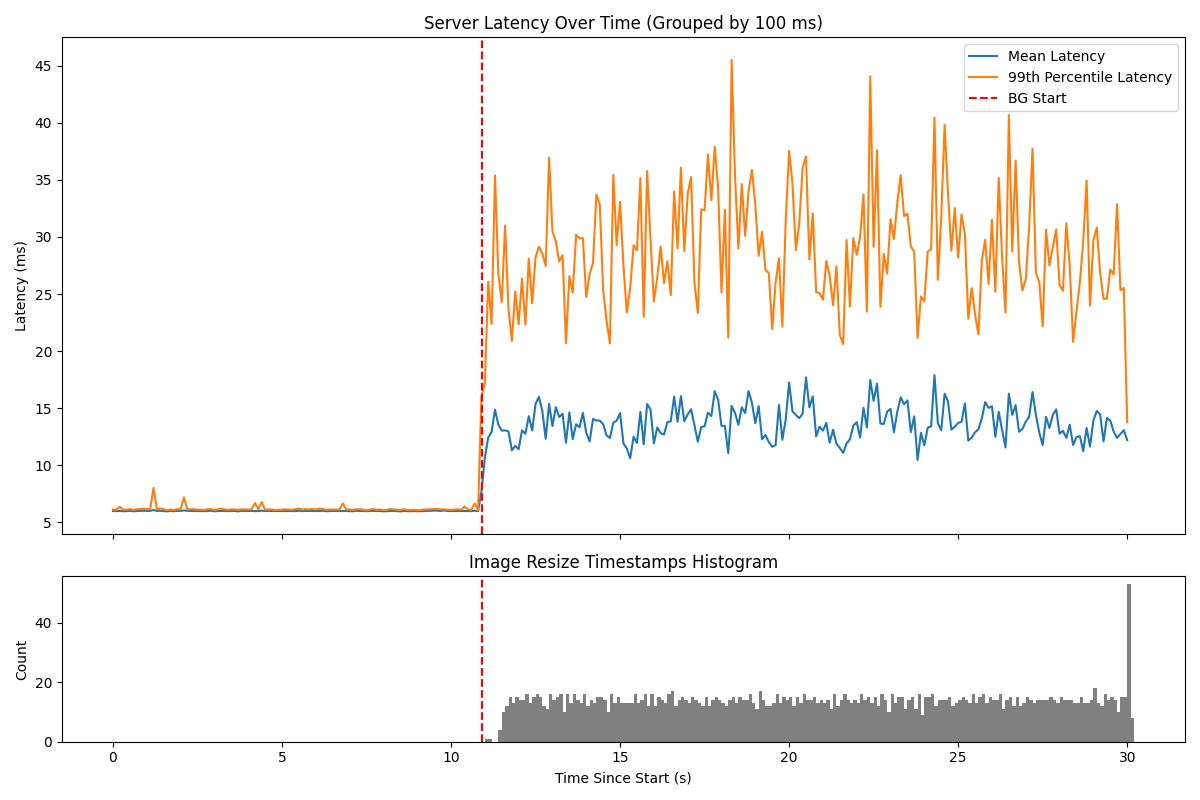
\includegraphics[width=\columnwidth]{graphs/srv-bg-weight-150-low.png}
        \caption{Low load stetting, utilization before starting the BE tasks is
        around 85\%}\label{fig:srv-bg-weight-150-low}
        \vspace{12pt}
    \end{subfigure}
    \hspace{\fill}
    \begin{subfigure}{\columnwidth}
        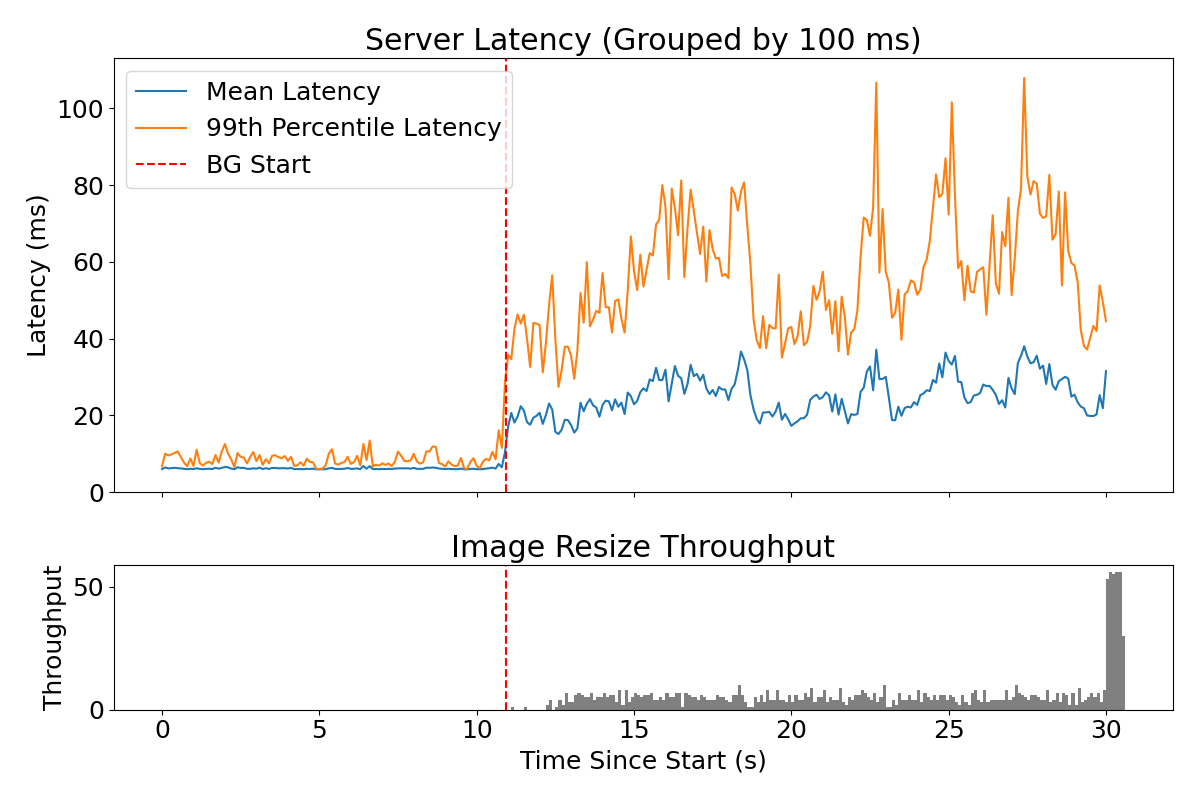
\includegraphics[width=\columnwidth]{graphs/srv-bg-weight-150-high.png}
        \caption{High load setting, utilization before starting the BE tasks is
        around 95\%}\label{fig:srv-bg-weight-150-high}
    \end{subfigure}
    \vspace{4pt}
    \caption{Latencies of the server and iteration counts of the background
    tasks in different load scenarios show the BE tasks interfering with the LC
    server. Note the different y axis limits. The upper graphs show end-to-end
    request latencies, and the bottom graph is a histogram of completed
    iterations of the BE tasks}\label{fig:srv-bg-weight-150}
\end{figure}

In order to understand why the jump in latency is happening when the BEs run, we
reproduce the effects in a simpler benchmark. The experiment shown in
\autoref{fig:kubernetes-weight-150} includes a complicated software stack of
Kubernetes, uvicorn, FastAPI, and Python. All of this has performance
implications, and we can see that even before the BE load starts there are large
latency spikes up to 30ms.

To exclude these effects, we run a simple CPU-bound server with a pool of worker
threads. We run an open-loop client on a remote machine, and then start two BE
workloads doing image resizing. We put the LC server and the BE resize job each
in their own \cgroups{} group with weights 150 and 1 respectively, and pin them
to the same set of cores. \autoref{fig:srv-bg-unedited} shows the result: we see
that at a $\sim$85\% baseline utilization of the server, after starting the BEs
the server's mean latencies spike up from steady at around 6ms to as high as
20ms, and much higher for 99th percentile latencies. At a baseline utilization
of 95\%, those numbers increase to up to 40ms for the the mean latency, and 80ms
for the tail.

\begin{figure}[t]
    \centering
    \begin{subfigure}{\columnwidth}
        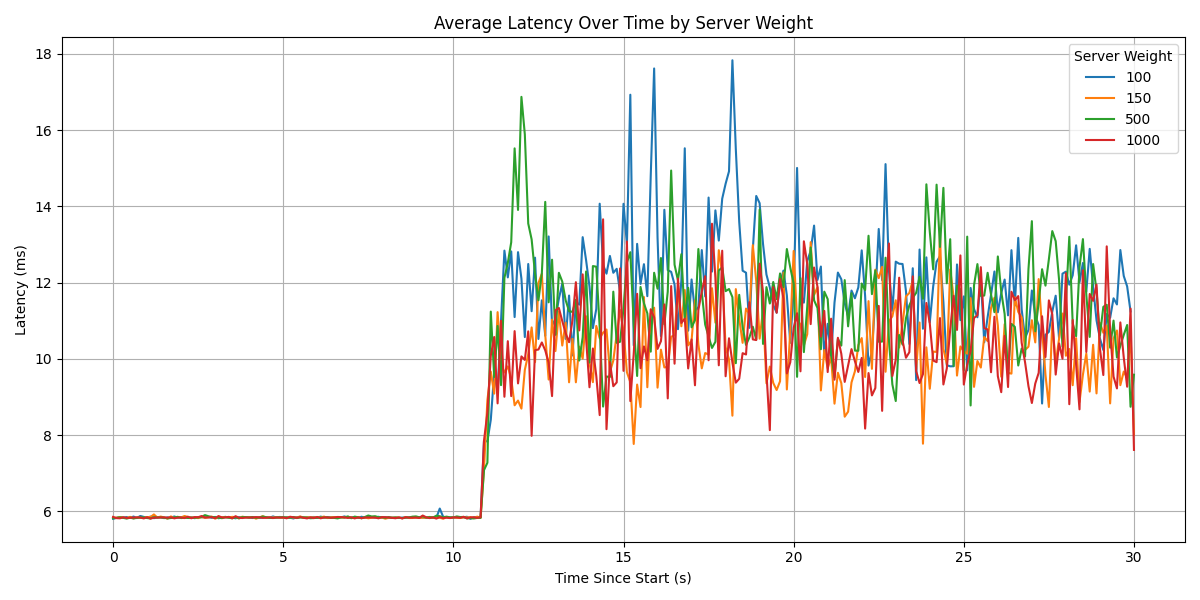
\includegraphics[width=\columnwidth]{graphs/srv-bg-weight-cmp-low.png}
        \caption{Low load stetting, utilization before starting the BE tasks is
        around 85\%}\label{fig:srv-bg-weight-cmp-low}
        \vspace{12pt}
    \end{subfigure}
    \hspace{\fill}
    \begin{subfigure}{\columnwidth}
        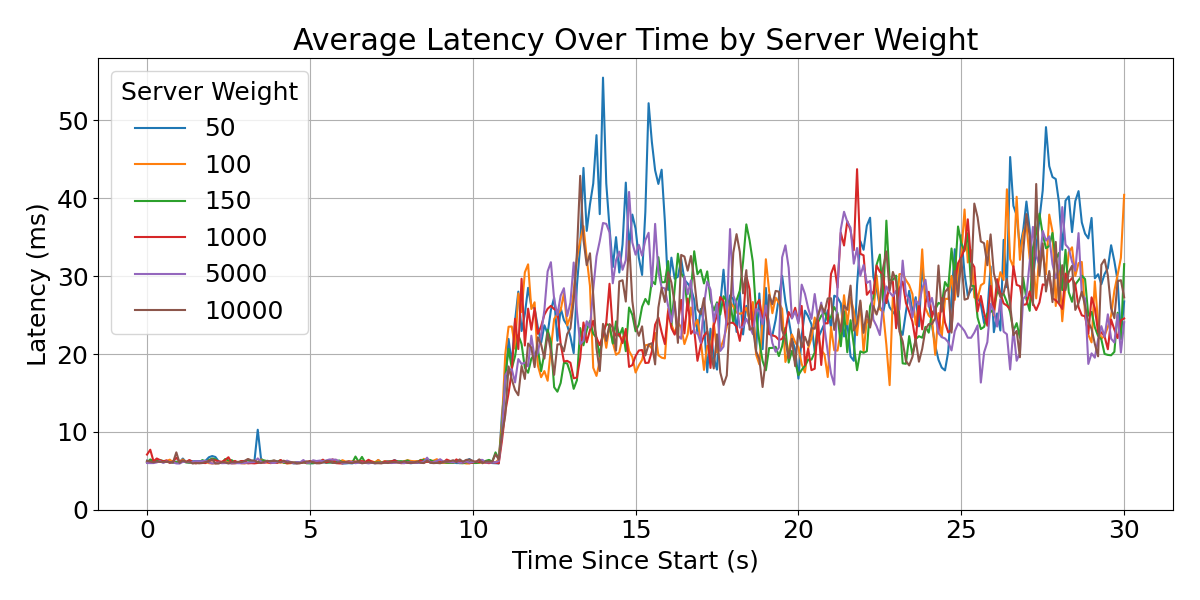
\includegraphics[width=\columnwidth]{graphs/srv-bg-weight-cmp-high.png}
        \caption{High load setting, utilization before starting the BE tasks is
        around 95\%}\label{fig:srv-bg-weight-cmp-high}
    \end{subfigure}
    \vspace{4pt}
    \caption{Latencies of the server and iteration counts of the background
    tasks in different load scenarios show the BE tasks interfering with the LC
    server. Note the different y axis limits. The upper graphs show end-to-end
    request latencies, and the bottom graph is a histogram of completed
    iterations of the BE tasks}\label{fig:srv-bg-weight-cmp}
\end{figure}

\cgroups{} supports weights in the range of [1,10000]; a possible explanation
could be that Kubernetes did not set the weights far apart enough. However,
running the same experiment with the server weight set to 1000 show the exact
same phenomenon. \autoref{fig:srv-bg-weight-cmp} shows the average server
latencies when running it with different weights; the BE task always has weight
1.

\begin{figure}[t]
    \centering
    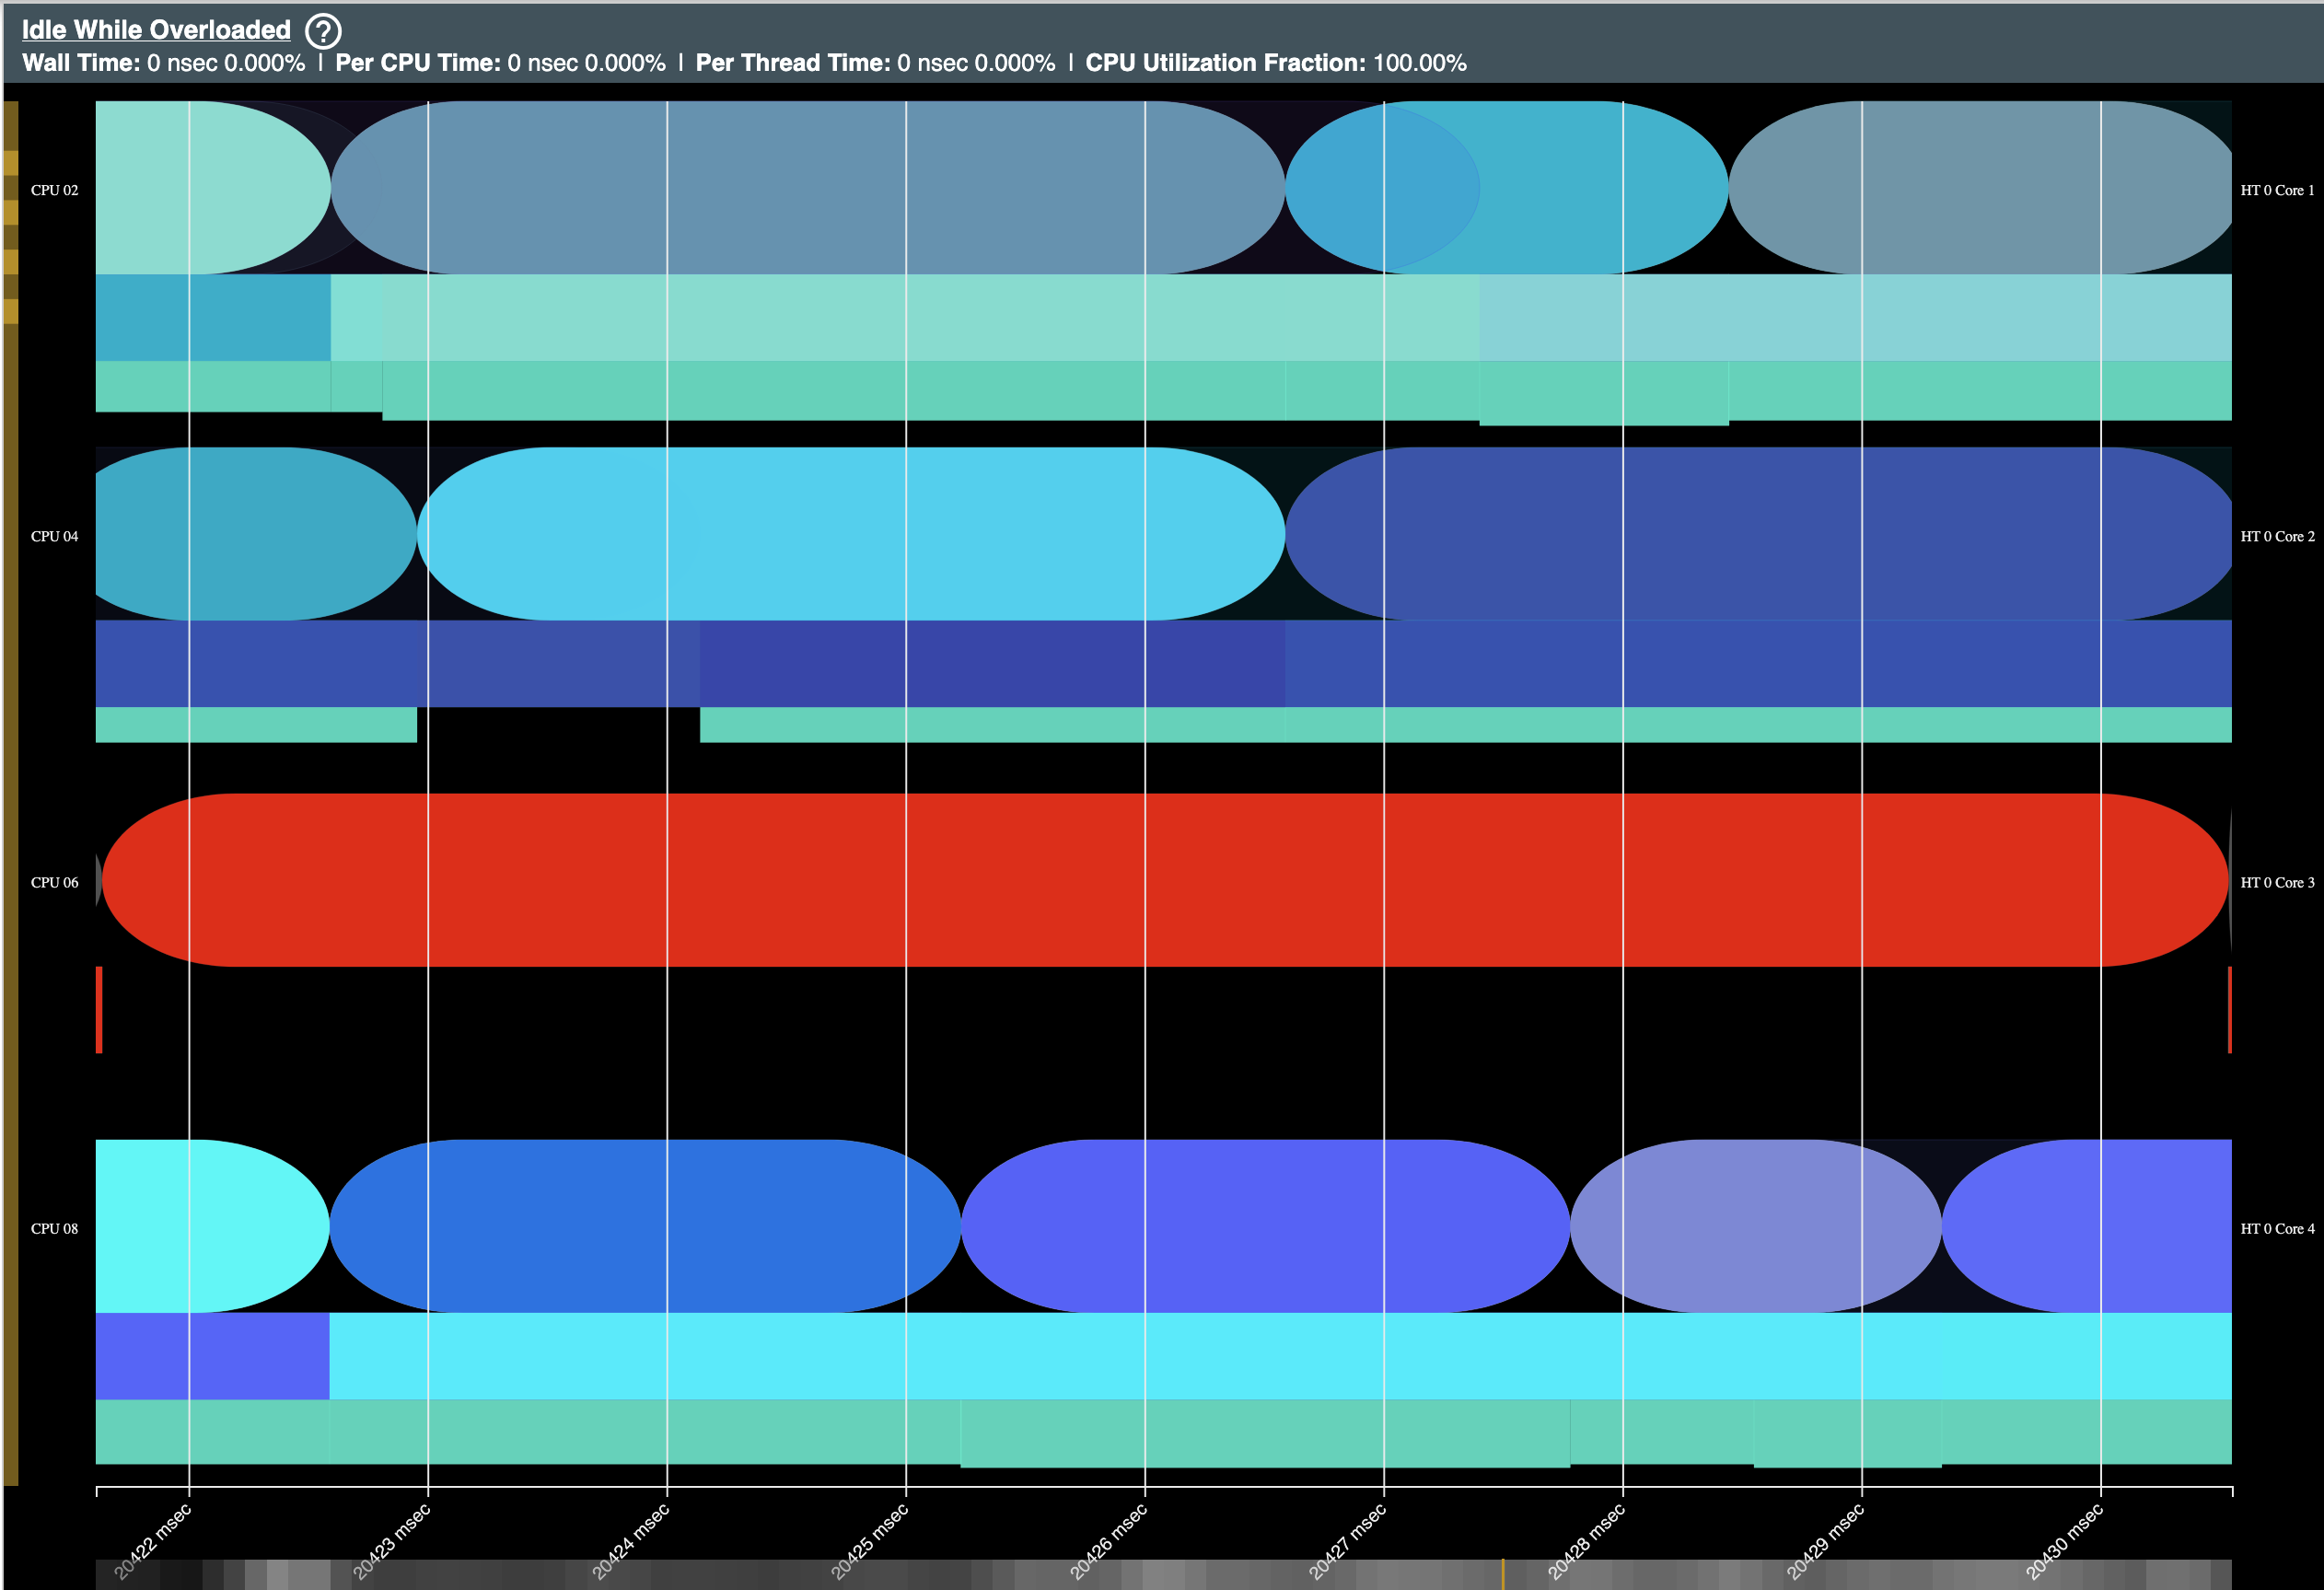
\includegraphics[width=\columnwidth]{graphs/schedviz-problem.png}
    \caption{The BE thread (red) runs on one core, while LC threads (shades of
    blue) are queued and waiting on other cores. Each thread is a different
    color, circles represent which thread is running on that core while
    rectangles underneath show waiting but runnable threads.
    }\label{fig:schedviz-problem}
\end{figure}

Using this simplified experiment, we analyze perf traces of the scheduling
decisions by visualizing the trace using schedviz~\cite{schedviz-tool}.
\autoref{fig:schedviz-problem} shows a 10ms outtake of the resulting image. The
process running on each core is shown as an oval, and queued processes are shown
as rectangles below; the x-axis is time and the y-axis shows the 4 cores the
experiment is running on. What we see is that \textit{one core is running a BE
process, while LC processes are queued on another}. On core 6, the red process
that is running for the whole 10ms is a BE process, while LC threads, shown in
varying shades of blue, are queued on the other cores.

\subsection{Weights are enforced only locally}\label{ss:problem:weights-local}

The reason this priority inversion is possible is that Linux maintains a
separate runqueue on each core, in order to avoid the overheads of accessing
global state for every scheduling decision. Within each runqueue, Linux's
scheduler works to maintain the correct ratio of received CPU time at each
scheduling; but Linux does not enforce the weight ratios across cores. This
leads to the above failure mode, where one core has no runnable high weight
processes and thus runs a low weight one, whereas another core has queued high
weight processes.

\subsection{Enforcing weights across cores is
hard}\label{ss:problem:cross-core-hard}

This is not just a poor implementation: a weight-based interface is at odds with
machine-wide policy enforcement. In order to strictly and globally enforce a
processes weight, the scheduler would need to compare different cores' runqueues
at every scheduling decision. This is because, in a weight-based system, the
definition of what process should be running changes over time. If a core has
one high-weight and one low-weight group, before running the low-weight group it
needs to know if any other cores have recently run a different process within
that group, because that would affect how much time it is owed on this core.

Managing and calculating global shares is complex: calculating whether a given
process is owed time globally requires knowing the total weight across all cores
as well as the sum of time that all the processes in the group have gotten. Such
a calculation would include complicated accounting that takes into account,
amount other things, different cores' virtual times, processes' weights, groups,
and limits. Just within runqueues the accounting is already so complicated that
comments in the Linux source include function derivations and equation
rewriting.

On top of that, enforcing weights across cores is expensive: looking at remote
queues at each scheduling decision removes the benefit of having local
runqueues. In increasingly multi-core and multi-NUMA machines, synchronization
is expensive; other work has found that kernel lock contention is a bottleneck
to performance at scale~\cite{afaas}. This means that the overheads of
maintaining a weight split as a global invariant can quickly become prohibitive.


\subsection{Weights interact poorly with tick-based
scheduling}\label{ss:problem:quantum}

Using very large weight differentials as an interface to isolate LC and BE
doesn't work well because preemption is tick-based. Even on a single runqueue,
in a weight based scheme BE processes get a fair share of the CPU. The problem
is that, when this happens, the BE process will interrupt any running LC process
for a whole tick. In Linux, hardware ticks are 4ms long. This means that an LC
thread processing a request may be interrupted for up to 4ms, provided the BE
process runs for that long before blocking. 4ms can be a large amount of time
for microservice workloads, whose SLOs are often in the low double digit or even
single digit ms realm.~\cite{in-the-plex, sigmaos}



